\subsection{Тематическое моделирование}

Для тематического моделирования в качестве модели используется латентное размещение Дирихле.

Для оценки качества данной модели используется перплексия (англ. \textit{perplexity}) --- оценка того, насколько хорошо вероятностная модель предсказывает выборку. Низкая перплексия указывает на то, что распределение вероятностей хорошо предсказывает выборку. 

В зависимости от параметра модели, отвечающего за количество тем у распределения текстов, получилась следующая зависимость значения перплексии от количества тем:


\begin{figure}[H]
\centering
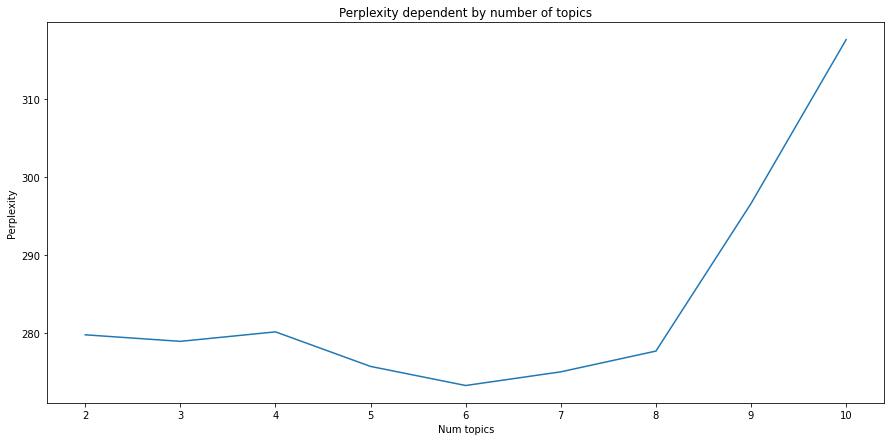
\includegraphics[scale=0.5]{pics/perplexity.png}
\caption{Перплексия модели в зависимости от количества тем в наборе Клинтон}
\end{figure}



Ниже приведены примеры слов, принадлежащие каждой из 6 (с оптимальным значением перплексии) тем:

\begin{table}[H]
\centering
\begin{tabular}{ | l | l | l | }
\hline
Номер темы & Слова \\ \hline
1 & obama, state, president, government, american, \\ & israel,  policy, country \\ \hline
2 & woman, say, work, health, year, senate, group, \\ & government,  support, company \\ \hline
3 & call, get, work, see, want, know, good, also, think, tomorrow \\ \hline
4 & secretary, office, state, meet, room, department,  \\ &  arrive, route, depart, private \\ \hline 
5 & state, information, benghazi, department, doc, case, subject, \\ & iran, agreement, house \\ \hline
6 & cheryl, gov, fyi, sullivan, state, friday, sunday, branch,  \\ & wednesday, april, january \\ \hline 
\end{tabular}
\caption{Полученное описание тем в наборе Клинтон}
\end{table}


Для визуализации работы алгоритмы используется представление тем в
\textit{2D}, то есть вычисляется двумерная проекция всех точек и
затем визуализируются эти два измерения, причем в интерактивном виде, что
позволяет нам получить представление, понятное человеку:



\begin{figure}[H]
\centering
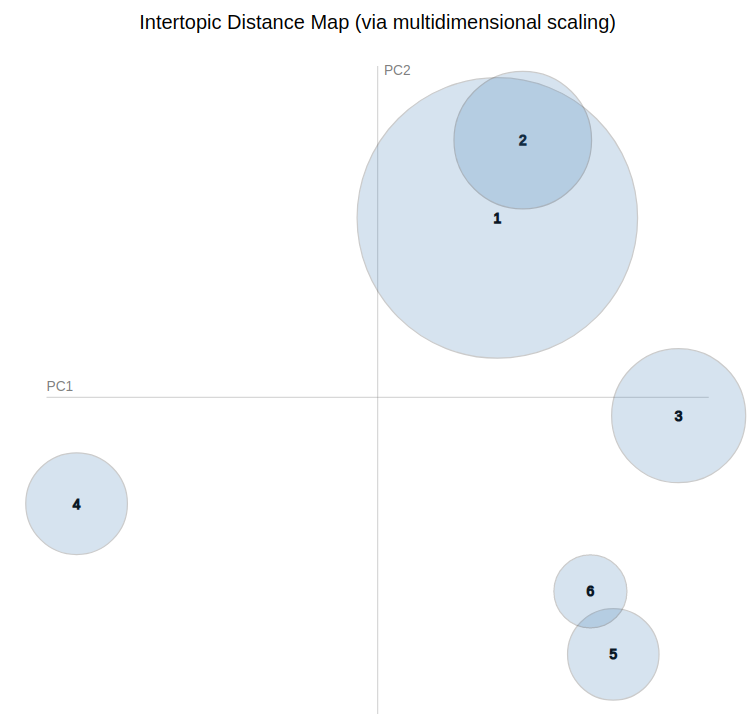
\includegraphics[scale=0.45]{pics/words_map.png}
\caption{Визуализации тем для модели латентного размещения Дирихле в наборе Клинтон}
\end{figure}
